\documentclass[../main.tex]{subfiles}
\graphicspath{{img},{img/ink},{ink}}

\begin{document}

\begin{tcolorbox}[
    width=\textwidth,
    height=\textheight,
    title=Versuch: Induktion bei Flächenänderung,
    fonttitle=\Large,
    before title=\vspace{0.2cm}, after title=\vspace{0.2cm},
    colback=white,
    title filled=true, 
    colbacktitle=mygray,
    colframe=black,
    coltitle=black,
    ]

    \vspace{0.2cm}
    \textbf{Klassenstufe}: 11/12

    \vspace{0.4cm}

    \textbf{Fachlicher Bezug}: Induktionsspannung, magnetischer Fluss
    \vspace{0.4cm}

    \begin{minipage}[c]{0.52\textwidth}
        \textbf{Material}:
        \vspace{-0.2cm}
        \begin{itemize}[noitemsep]
            \item Neva-Spule
            \item Schrittmotor + Umlenkrolle
            \item Rechteckrahmen $n=500$ Windungen
            \item stabilisierendes Netzgerät 300 V 
            \item Amperemeter + Voltmeter
            \item Stativmaterial
            \item Sicherheitskabel
        \end{itemize}
    \end{minipage}
    \hspace{0.3cm}
    \begin{minipage}[c]{0.48\textwidth}
        \centering
        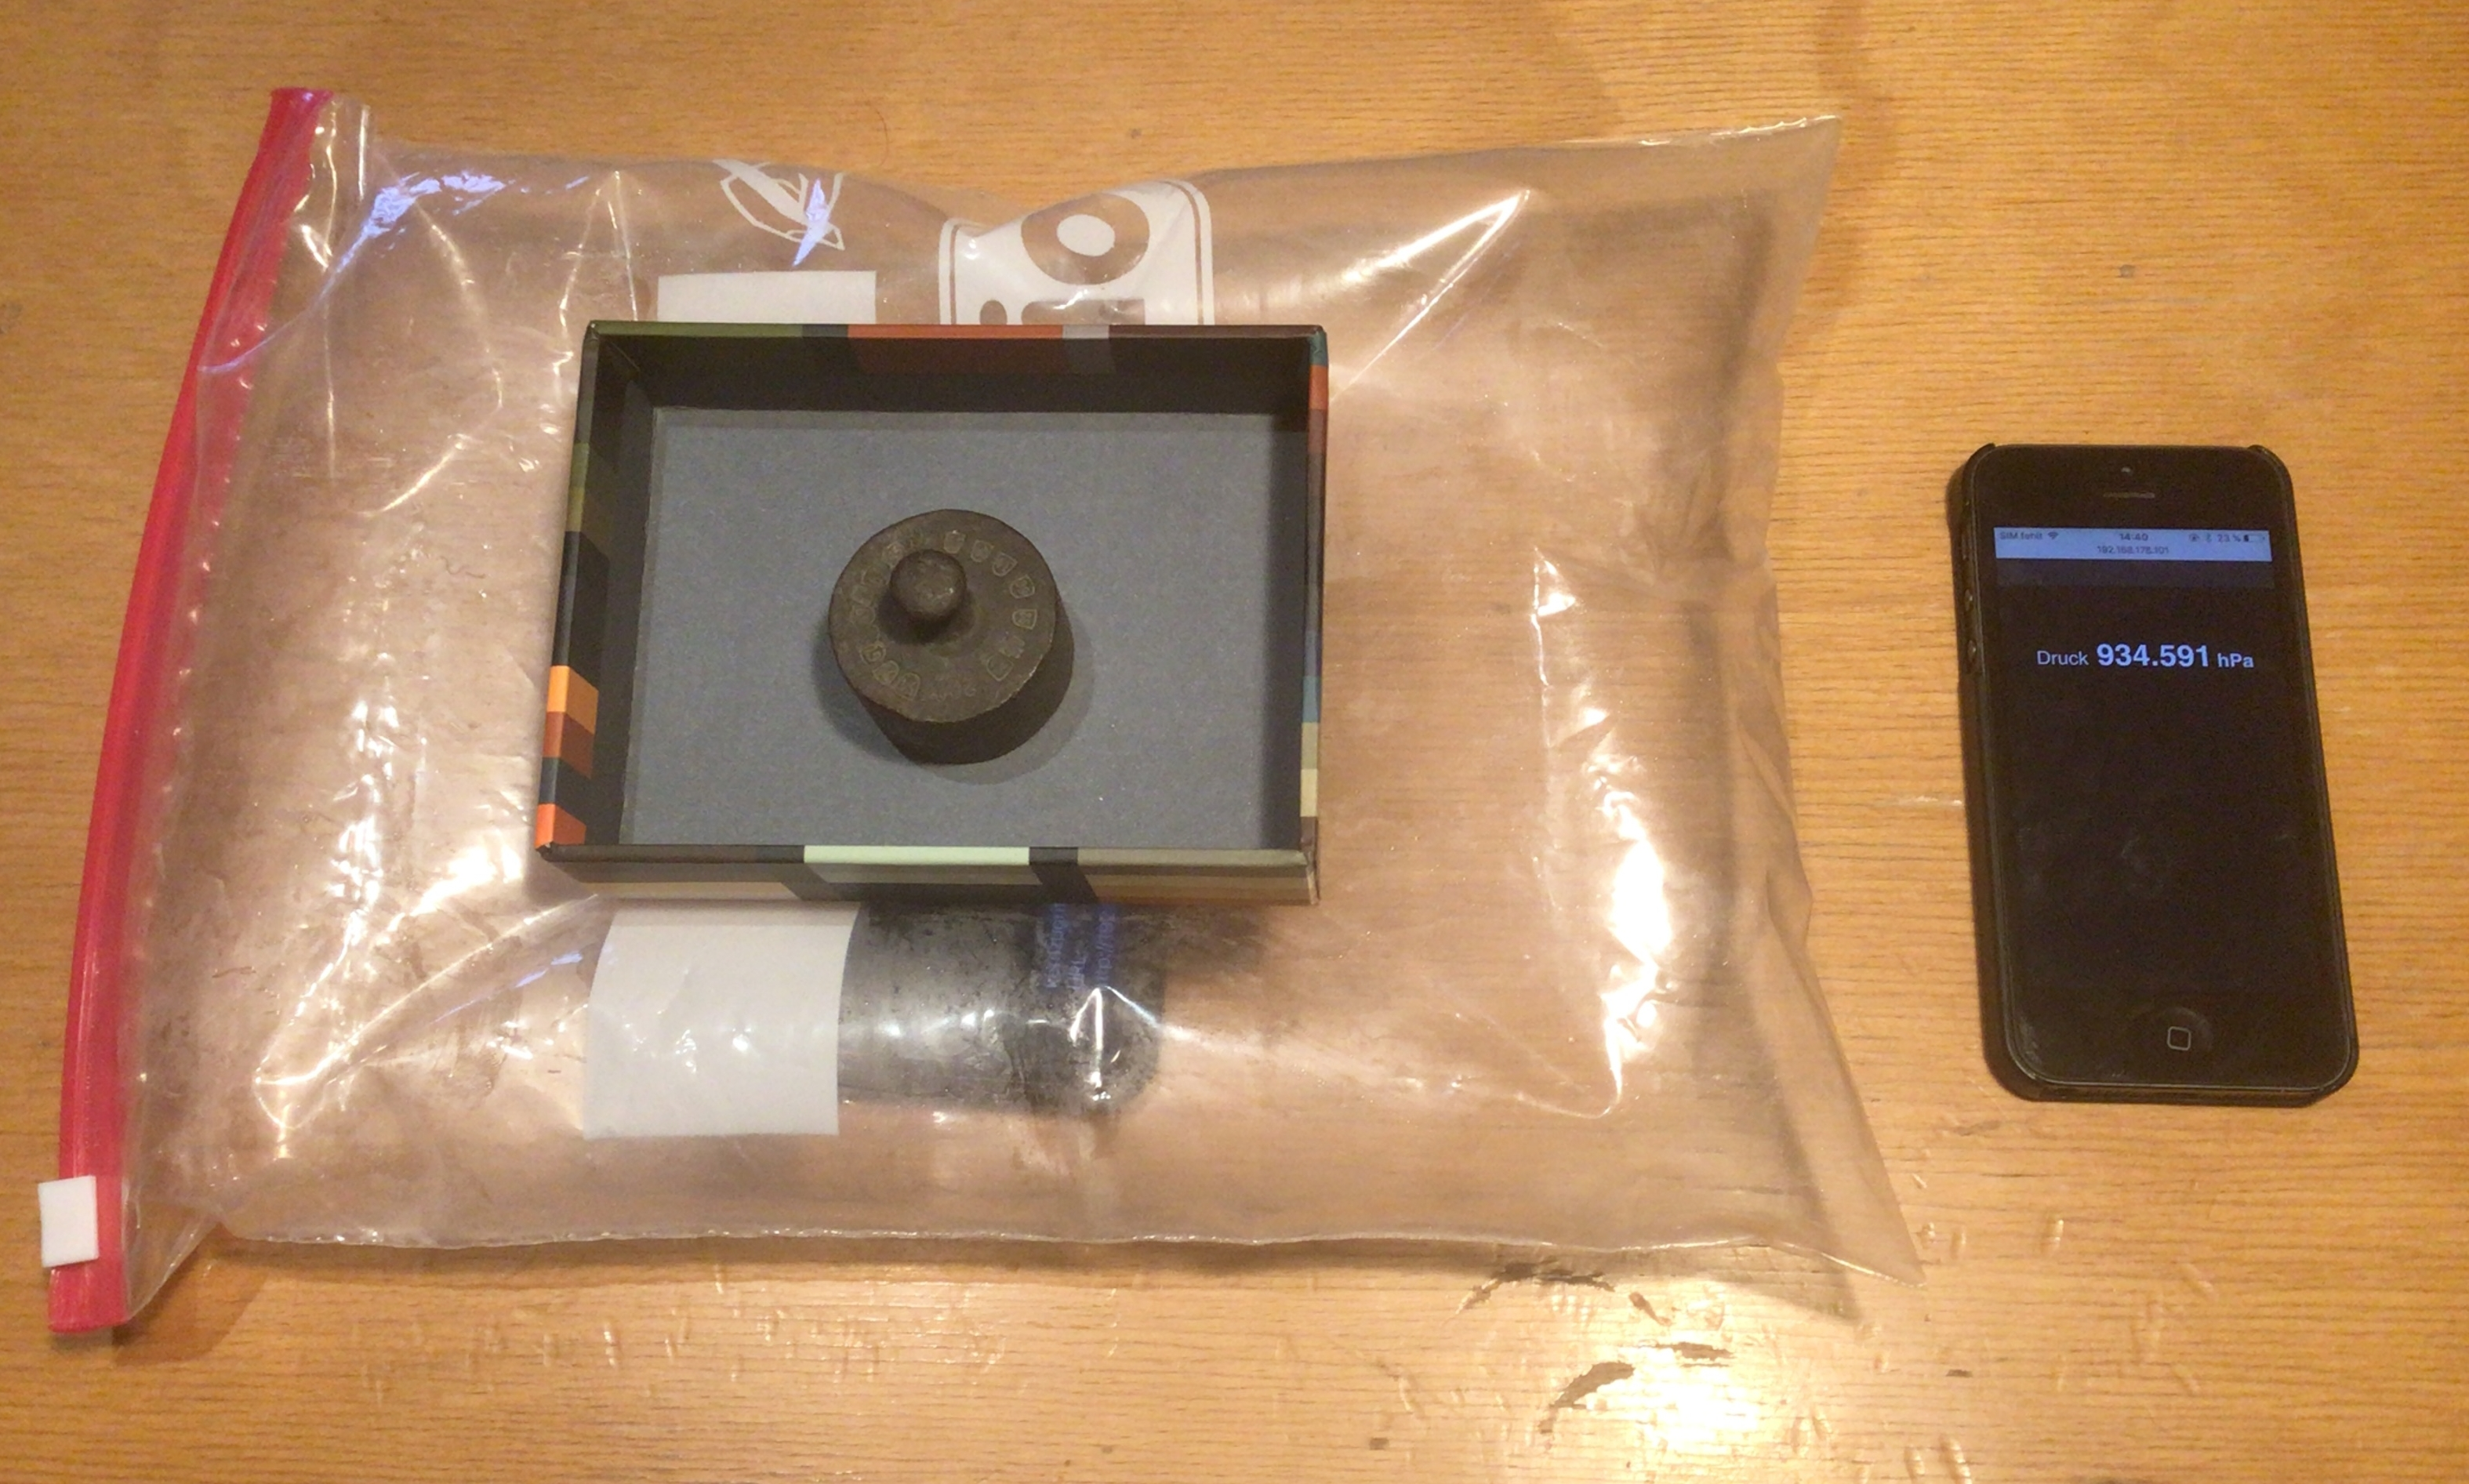
\includegraphics[width=0.85\textwidth]{img/versuchsaufbau}
    \end{minipage}

    \vspace{0.5cm}
    \textbf{Aufbau}: Ein stabilisierendes Netzgerät dient als Spannungsquelle für die Neva-Spule. Zur Messung der Stromstärke durch die Spule wird ein Amperemeter in Reihe geschaltet. Über einen Schrittmotor und eine Umlenkrolle kann die Position des Rechteckrahmens in der Spule kontrolliert werden. An den Rechteckrahmen wird ein Spannungsmessgerät angeschlossen.  

    \vspace{0.4cm}
    \textbf{Durchführung}: Über die Strombegrenzung des Netzgeräts wird eine Stromstärke $I=100$ mA durch die Spule eingestellt. Die Schnur des Rechteckrahmens wird am Schrittmotor um verschieden große Durchmesser auf- bzw. abgewickelt. Dadurch lässt sich der Rahmen mit verschiedenen Geschwindigkeiten in die Spule einführen (Fläche $A$ nimmt zu) und anschließend wieder herausheben (Fläche $A$ nimmt ab).

    \vspace{0.4cm}
    \textbf{Ergebnis}: Zur Herleitung der Induktionsspannung $U_{\text{ind}}$ wird die Wirkung des magnetischen Flusses $\phi$ aus zwei getrennten Beobachtungen gewonnen:
    \begin{align*}
        U_{\text{ind}}=-n \cdot \underbrace{(\dot{A}\cdot B+ A\cdot \dot{B})}_{\dot{\phi}}
    \end{align*}
    In diesem Versuch wird der erste Beitrag $U_{\text{ind,1}}=-n\cdot \dot{A} \cdot B$ untersucht. Man beobachtet die Proportionalität $\Delta U_{\text{ind,1}} \sim -\dot{A}$. \\
    Senkt man den Rahmen in die Spule, liegt eine positive Änderung der Fläche vor und eine negative Induktionsspannug wird gemessen.\\
    Hebt man den Rahmen aus der Spule, liegt eine negative Änderung der Fläche vor und eine positive Induktionsspannung wird gemessen. 

    \vspace{0.4cm}
    \textbf{Didaktische Bemerkungen}: Um die Abhängigkeit von der Windungszahl $n$ aufzuzeigen, werden bei konstanter Flächenänderung und konstantem Magnetfeld verschiedene Rechteckrahmen eingesetzt.  

    \vspace{0.4cm}
    \begin{minipage}[c]{0.85\textwidth}
        \textbf{Bemerkungen}: Da ein Netzteil mit Hochspannung eingesetzt wird, ist auf die Verwendung von entsprechenden Sicherheitskabeln zu achten.\\
        Der Rechteckrahmen sollte mindestens $n=500$ Windungen besitzen, da ansonsten die Stromstärke im Rahmen zu hohe Werte annimmt.
    \end{minipage}
    \hspace{0.5cm}
    \begin{minipage}[c]{0.1\textwidth}
        \centering
        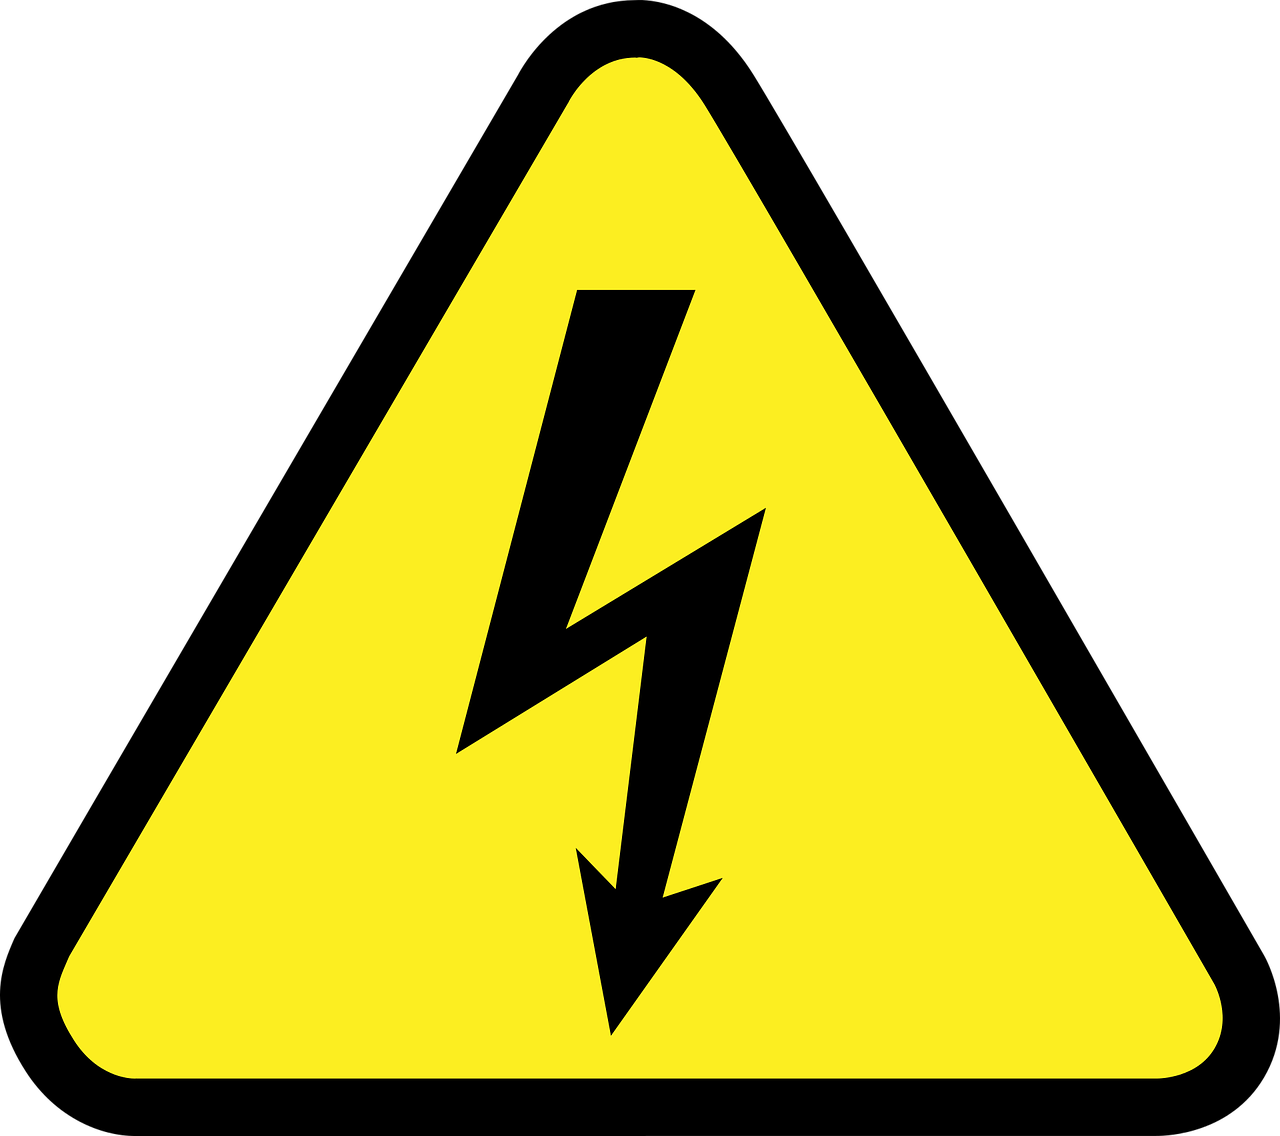
\includegraphics[width=1\textwidth]{img/hochspannung}
    \end{minipage}

\end{tcolorbox}
\end{document}
